\documentclass[runningheads]{llncs}
% Packages
\usepackage[T1]{fontenc}
\usepackage{graphicx}
\usepackage{natbib}
%
\begin{document}
% Page 1
\title{PhageLysin: Phage Endolysin Finder}
%
\author{Tiago Baptista\inst{1} \and
Hugo Oliveira\inst{2} \and
Óscar Dias\inst{2}}
%
\institute{University of Minho, Portugal \and
University of Minho, Center of Biological Engineering (CEB), Portugal}     
%
\maketitle
%
%\begin{abstract}
%Insert abstract here
%\end{abstract}
%
\section{Introduction}
%
\subsection{Aims}
Bacterial multidrug resistance to antibiotics is one of the most concerning problems faced in modern days, however new alternative therapies are being developed. The potential use of enzybiotics, a relatively new term that defines therapies using phage-encoded enzymes, normally phage lytic enzymes, is rising as arguably the best alternative to regular antibiotics. One of those enzymes is the endolysin, utilized by phages to degrade the cell wall from within. There are also several studies that have shown that recombinant endolysins can also be applied to degrade cell wall from the outside, thus confirming their antibacterial properties \cite{Abdelrahman2021} \cite{Briers2019}.

This project aims at building a comprehensive database of phage endolysins. The ultimate goal, probably outside of the scope of this project, would be the development of a machine learning (ML) tool to provide a quick and reliable way to identify endolysins in new phage genomes, but also on metagenomic sequencing data.
The main steps of this project include: (i) review of public datasets containing metagenomic data; (ii) review of annotation tools applied to phage genomes on metagenomic data; (iii) build a database of phage endolysins; (iv) explore ML approaches to improve the accuracy of predictions i.e. classify endolysins.
%
\subsection{Phages and endolysins}
Phages represent the most plentiful and varied biological entities on the planet and are thought to exist in virtually every imaginable environment. It is estimated that there are \(10^{31}\) phages, outnumbering their bacterial hosts by an estimated tenfold \cite{Dion2020} \cite{Oliveira2013} \cite{Sharma2017}. Phages exhibit remarkable diversity with a wide range of genome sizes from as low as 2,435 bp to as high as >540 kb \cite{Dion2020}.

Phages classification is based on various characters that describe the virus and allow to differentiate one from another. Characters include the molecular composition of the genome; the structure of the virus capsid and whether or not it is enveloped; the gene expression program used to produce virus proteins; host range; pathogenicity; and sequence similarity. Even though all characters are important in determining taxonomy, sequence comparisons using both pairwise sequence similarity and phylogenetic relationships are the main sets of characters to define and distinguish virus taxa \cite{Lefkowitz2018}.
Furthermore, phages taxonomy is a complex subject and is regularly under revision by the International Committee on Taxonomy of Viruses (ICTV) \cite{Walker2022}. A recent ICTV taxonomy update constituted the class \textit{Caudoviricetes} as one of the most important ones, encompassing all tailed bacterial and archaeal viruses with icosahedral capsids and a doublestranded DNA (dsDNA) genome \cite{Turner2023}.

Phages replication first requires infection of the bacteria so they must bind to the bacterium surface and subsequently resort to a spike shaped complex of proteins at the bottom of the baseplate of phage's structure that punctures into the bacterial host, allowing a release of phage's genetic material into the host's intracellular environment.
After that, phages can undergo one of two possible life cycles: lytic or lysogenic. 
The lytic cycle is followed by strictly lytic phages (also termed virulent phages) and consists in the seizure of bacterial host's metabolic machinery, which is first redirected to replication of phage's genome to create multiple copies of its own genetic material. Then, translation occurs and the synthesis of viral proteins and enzymes is achieved. Among them, some are used to assemble capsid and tails of new phages and package their genome, while enzymes such as holins and endolysins allow bacterium lysis and newly assembled phages release.
In turn, the lysogenic cycle exhibited particularly by temperate phages requires the integration of the viral genome within the host's genome. This lysogenic bacteria has an integrated prophage within its genome, that can remain dormant through numerous bacterial cell divisions, unless triggered by stress or cellular damage in the bacterial host. Upon activation by these factors, the phage cycle shifts towards replication through a lytic pathway, after excision from the bacterial genome, culminating in the release of the new phage particles \cite{Harada2018} \cite{Sharma2017}. 

It is thought that the holin-endolysin lytic system, also known as the lambda paradigm is universal in almost all dsDNA phages. As depicted in Fig.~\ref{fig1}, this system consists of endolysin accumulation in the intracellular space due to the bacterial inner membrane. This accumulation goes on until the holin, a small hydrophobic membrane-spanning protein, after being expressed at a genetically programmed time, had accumulated in clusters producing homo-oligomeric pores in the inner membrane. Holin hole formation triggers the activation of the endolysin by granting its access to the peptidoglycan (PG) (or murein), a heteropolymer consisting of disaccharidepeptide repeat units linked by glycosidic bonds that form glycan strands. These strands are cross-linked through pentapeptides by 4–3 and 3–3 linkages. Endolysin muralytic activity i.e. its capability to degrade the PG, results in a unsustainable internal osmotic pressure, leading to cell lysis and progeny release. \cite{Cahill2019} \cite{Oliveira2013}. Endolysins classification based on their lytic activity can be categorised into glycosidases, amidases and endopeptidases \cite{Abdelrahman2021} \cite{Oliveira2013} as shown in Fig.~\ref{fig1}.

Endolysins unique ability to rapidly kill bacteria in a species specific manner puts them as promising antibacterial and biocontrol agents with applications in fermentations, food preservation, biotechnology, and medicine.
Studies regarding endolysin capacity to lyse bacteria when externally added were already performed. In the case of Gram-positive bacteria, cell lysis was already achieved \textit{in vitro}, leading to the complete death of a streptococcus culture in a few seconds \cite{Oliveira2013}. Other \textit{in vivo} studies have shown endolysins efficacy against a variety of Gram-positive bacteria such as PlyC, C1, ClyR, Cpl-1, ClyV, and ClyJ \cite{Abdelrahman2021}.
Regarding Gram-negative bacteria, exogenous action of endolysins is still restricted due to the presence of the impermeable OM, constituting one of the most important challenges in endolysin therapy, however in recent years molecular engineering
approaches have increased the applicability of endolysins in targeting Gram-negative bacteria \cite{Abdelrahman2021} \cite{Oliveira2013}.

\begin{figure}
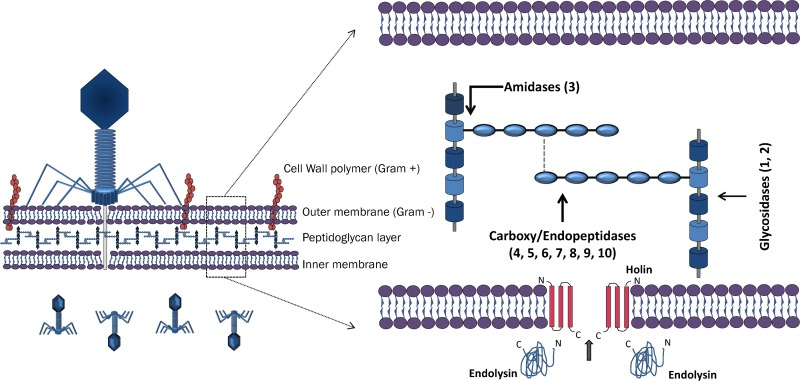
\includegraphics[width=\textwidth]{holin-endolysin-system.jpg}
\caption{Schematic representation of phage endolysins access to the PG through the holin-endolysin lytic system, alongside with a generic PG structure illustration of endolysins cleavage sites \cite{Oliveira2013}.} \label{fig1}
\end{figure}

\subsection{Phages and metagenomics}
The nonexistence of a conserved genetic marker combined with the predicted large number of existing phages makes phage genomic diversity really difficult to comprehend \cite{Dion2020}. Viral metagenomics emerged as a means to assess phage diversity and indirectly abundance \cite{Clokie2011}, overcoming culture-based approaches and single marker genes challenges \cite{Dion2020}. This approach consists of collecting, concentrating and sequencing the total viral component/population from a specific environment \cite{Clokie2011} \cite{Hatfull2011}. This became possible due to optimization of required steps to obtain good quality viral nucleic acids, progress in sequencing technologies combined with more affordable costs and the rise and improvement of a set of analytical tools, allowing the construction of large-scale viral datasets of viral communities \cite{Dion2020}.

Metagenomics can be used to identify phages sequences and phage genes with higher or lower expression in a specific environment, which provides a good entry point to understand phages roles and reducing the need to culture phage hosts and isolate phages. It can also provide information on phages not prone to propagation, or phages with hosts that cannot be cultured in the lab \cite{Clokie2011}. 
%
\section{Materials and Methods}
%
\subsection{Phage endolysins database}
We expect to build a solid endolysins database that can be used to train the machine learning models, by querying existing databases containing endolysins.

Phage lytic proteins databases containing endolysins are available, namely phiBIOTICS \cite{Hojckova2013}, EnzyBase (renamed to EnzyBase2) \cite{Wu2012}, GMEnzy \cite{Wu2014}, PhaLP \cite{Criel2021} and PhalydDB \cite{Gou2022}.
phiBIOTICS, EnzyBase2 and GMEnzy data is collected manually so they naturally have few entries. Oppositely, PhaLP and PhalydDB are comprehensive databases with PhaLP being automatically updated with each new UniProt release, thus containing a significantly bigger amount of entries \cite{Criel2021} \cite{Gou2022}.
It would be possible to construct the endolysins database by querying the previously mentioned databases. PhaLP allows database querying on MySQL \cite{Criel2021}. phiBIOTICS, EnzyBase2 and GMEnzy are not optimised for that so manual retrieving of information, use of APIs or web scraping could be possible ways to query these databases. PhalydDB is still a recent project with \cite{Gou2022} having a data sharing statement indicating the necessity to request their authors access to their data.

Even though it is not a specialized database for phage lytic proteins, endolysins can be queried from National Center for Biotechnology Information (NCBI)’s Protein database, for example using the Biopython package, thus providing an alternative way to build or complete the endolysins database.
%
\subsection{Metagenomic datasets}
With the rise of culture independent approaches, a great quantity of phage metagenomic datasets has emerged. In the scope of this project, we will review some of them that constitute potential usable datasets for our work.

In a study by Fernandez-Ruiz and collaborators \cite{Fernandez-Ruiz2018} a database of uncultured viral genomes was compiled from various sources. The dataset comprised 183,298 genomic sequences of uncultured viral genomes and they also compiled metadata associated with those sequences. Nayfach and collaborators \cite{Nayfach2021} performed a large-scale identification
of viral genomes from 11,810 bulk metagenomes from human stool
samples obtained from multiple studies. With these data they built the Metagenomic Gut Virus (MGV) catalogue gathering an astonishing 189,680 viral draft genomes. In this work of Camarillo-Guerrero and collaborators \cite{Camarillo-Guerrero2021} they introduce the Gut Phage Database, with approximately 142,000 non-redundant viral genomes gathered from a dataset of 28,060 global human gut metagenomes and 2,898 reference genomes of cultured gut bacteria. Roux and collaborators \cite{Roux2015} mined the viral signal from 14,977 publicly available bacterial and archaeal genomic datasets using VirSorter and yielding 12,498 high-confidence viral sequences with known hosts. Paez-Espino and collaborators \cite{Paez-Espino2016} analysed metagenomic sequence data from 3,042 geographically diverse samples uncovering over 125,000 partial DNA viral genomes. Coutinho and collaborators \cite{Coutinho2017} reported a dataset of 27,346 marine virome contigs that included 44 complete genomes of phages from marine environments. 
%
\subsection{Annotation tools applied to phages genomes on metagenomic data}
Fernandez-Ruiz and collaborators \cite{Fernandez-Ruiz2018} were able to identify putative endolysins using a database of uncultured viral genomes, alongside with related available metadata and a dataset of endolysin sequences. They used Prodigal \cite{Hyatt2010} on metagenomic mode to identify protein encoding genes of uncultured phage
genomes. Then, queried predicted protein sequences against the reference endolysin database using Diamond \cite{Buchfink2015}. To filter results and determine putative endolysins, they applied the following thresholds: identity $x \geq y$ 50\%, e-value $x \leq y$ 0.001, query coverage $x \geq y$ 30\%, and alignment length $x \geq y$ 50 amino
acids. They queried sequences against the Pfam database using HMMER version v3.1b2 \cite{Finn2015} with default parameters to identify protein domains and used SignalIP \cite{Petersen2011} to detect signal peptide sequences. 
This work could be of great importance to our project, because it provides a replicable methodology to identify putative endolysins in phage/viral genomes, by using our future built endolysins database and 
a selected metagenomic dataset with phage genomes. 

Despite that, it would also be necessary a way to identify phage genomes in metagenomic data.
Luckily, there are a great variety of tools to identify phages on metagenomic sequencing data. Ho and collaborators performed a comparative analysis on 10 tools with such purpose, namely DeepVirFinder, Kraken2, MetaPhinder, PPR Meta, Seeker, ViralVerify, VIBRANT, VirFinder, VirSorter and VirSorter2. Results suggested that Kraken2 should be considered to identify previously characterised phages, while for novel phage detection Kraken2 should be used in combination with tools such as VirSorter2 and DeepVirFinder.

Furthermore, we are still missing phage genome annotation tools to retrieve features to use on the ML models. MetaPhage \cite{Pandolfo2022} is a fully automated computational pipeline for phage detection, classification, and quantification of metagenomics data. It was designed for scalability and reproducibility, while it is modular, allowing users to only perform certain chunks of the pipeline. These characteristics are very interesting, because they could allow the usage of this pipeline for annotation purposes only. On top of that, it incorporates previously referred tools.
%
\subsection{Machine learning approaches to improve the accuracy of predictions i.e. classify endolysins}
ML approaches provide a promising way not only to predict phage virion proteins, but also their functions.
Nami and collaborators \cite{Nami2021} conducted a review on 10 different ML models for the previous purposes. The list of the models, alongside with the respective methods and features is presented in Table~\ref{tab1}. Table~\ref{tab1} also shows diversity regarding ML methods and features, allowing flexibility when choosing the ML model(s) for the scope of this project. Nevertheless, models performances must be evaluated in the context of our work, to allow for a weighted decision of a model in detriment of another.

\begin{table}
\caption{ML models and respective methods and features. \cite{Nami2021}.}\label{tab1}
\resizebox{\textwidth}{!}{%
\begin{tabular}{|l|l|}
\hline
Predictor & Method\\
\hline
ANN & “ACC, protein isoelectric Points” + ANN\\
Naïve Bayes & “ACC, DPC” + CFS + Naïve Bayes\\
PVPred & g-gap DPC + ANOVA+SVM\\
PhagePred & g-gap DPC + ANOVA + Multinomial Naïve Bayes + ANN\\
PVP-SVM & “AAC, ATC, CTD, DPC, PCP” + RF-based feature selection + SVM\\
SVM-based & g-gap DPC + “ANOVA, mRMR” + SVM + ANN\\
Ensemble RF & “CTD, bi-profile Bayes, PseAAC, PSSM” + Relief + RF + ANN\\
Pred-BVP-Unb & CT, SAAC, bi-PSSM+SVM + ANN\\
PVPred-SCM & DPC + SCM + ANN\\
Meta-iPVP & Probabilistic feature+SVM + ANN\\
\hline
\end{tabular}
}
\textit{SCM} scoring card method, \textit{SVM} support vector machine, \textit{AAC} amino acid composition, \textit{ATC} atomic composition, \textit{bi-PSSM} bi-profile position specific scoring matrix,
\textit{CTD} chain-transition-distribution, \textit{CT} composition and translation, \textit{DPC} dipeptide composition, \textit{GDPC} g-gap dipeptide composition, \textit{PCP} physicochemical properties,
\textit{SAAC} split amino acid composition, \textit{TR} training dataset, \textit{TS} testing dataset
\end{table}

In a recent work, Vieira and collaborators \cite{Vieira2023} developed the first ML tool to identify phage depolymerases. This tool is based on two algorithms, SVMs and ANNs that were used to train the machine learning models. This groundbreaking study shows immense progress in ML tools to identify phage lytic enzymes providing valuable insights for the future development of a ML tool to predict endolysins.
%
\bibliographystyle{plain}
%\bibliographystyle{plainnat}
\bibliography{references}
%
\end{document}


